\documentclass[25pt, a0paper, portrait]{tikzposter}

\usepackage{graphicx}
\usepackage{wrapfig}
% Atkinson Hyperlegible: accessibility-focused sans-serif (named in the
% RSECon26 accessibility guidance). Type1 package, works with pdflatex;
% part of texlive-fonts-extra / TeX Live 2023+ / MiKTeX.
\usepackage[sfdefault]{atkinson}
\usepackage[fontsize=28pt]{fontsize}
% \usepackage{microtype}  % conflicts with hyperref and tikzposter, see https://tex.stackexchange.com/questions/481636/incompatibility-between-tikzposter-class-microtype-and-hyperref-package
\usepackage{hyperref}

% \title{The Journal of Open Source Software}
% \author{\emph{EditorsWarrick Ball}
% \date{\today}
% \institute{University of Birmingham}
% \usetheme{Simple} % Default, Rays, Basic, Simple, Envelope, Wave, Board, Autumn, and Desert
% \usecolorstyle{Denmark}
% \titlegraphic{logo_large.png}
\settitle{}

% https://tex.stackexchange.com/questions/254257/tikzposter-and-doi-package-conflict
\def\HyperFirstAtBeginDocument#1{#1}
\begin{document}

% Title block with title, author, logo, etc.
% \maketitle

\makeatletter
    \setlength{\TP@blocktop}{.485\textheight}
\makeatother

% https://github.com/openjournals/joss/blob/main/public/logo_large.jpg
% logo, QR code

\block{}{
  \begin{center}
    \includegraphics[width=0.65\textwidth]{joss-logo-transparent-crop.png} \\
    \textbf{Editorial board} \\
    Arfon Smith (Editor-in-Chief),
    Warrick Ball,
    Matthew Feickert,
    Samuel Forbes,
    Daniel S.~Katz, \\
    Rachel Kurchin,
    Kevin M.~Moerman,
    Kyle Niemeyer,
    Kristen Thyng,
    Chris Vernon, and 102 editors
  \end{center}
}

\begin{columns}
\column{0.5}
%
\block{About}{
  The \href{https://joss.theoj.org/}{Journal of Open Source Software (JOSS)}
  is an academic journal (ISSN 2475-9066) publishing short articles about
  open source software with a research application at \url{joss.theoj.org/}. \\[0.5em]
  %
  Following \textbf{submission} an editor conducts \textbf{pre-review} triage to ensure the software is
  within scope.  Submissions passing this stage move to \textbf{review} where volunteers
  check functionality and that the software
  \href{https://joss.readthedocs.io/en/latest/review_checklist.html}{meets
  modern standards} --- documentation, tests, community guidelines. 
  All of this takes place on the
  \href{https://github.com/openjournals/joss-reviews}{openjournals/joss-reviews}
  GitHub repository in an open, iterative conversation with the authors.\\[0.5em]
  %
  JOSS gives software creators a \textbf{citable artefact} recognising their research
  contribution, and \textbf{encouraging good software practices}.  For Research Software
  Engineers in particular, it offers a route to formal, citable recognition in
  peer-reviewed literature.
}

\block{Publication statistics}{
  JOSS has \textbf{published over 3,600 papers} across a variety of research fields since 2016.
  %
  \begin{center}
    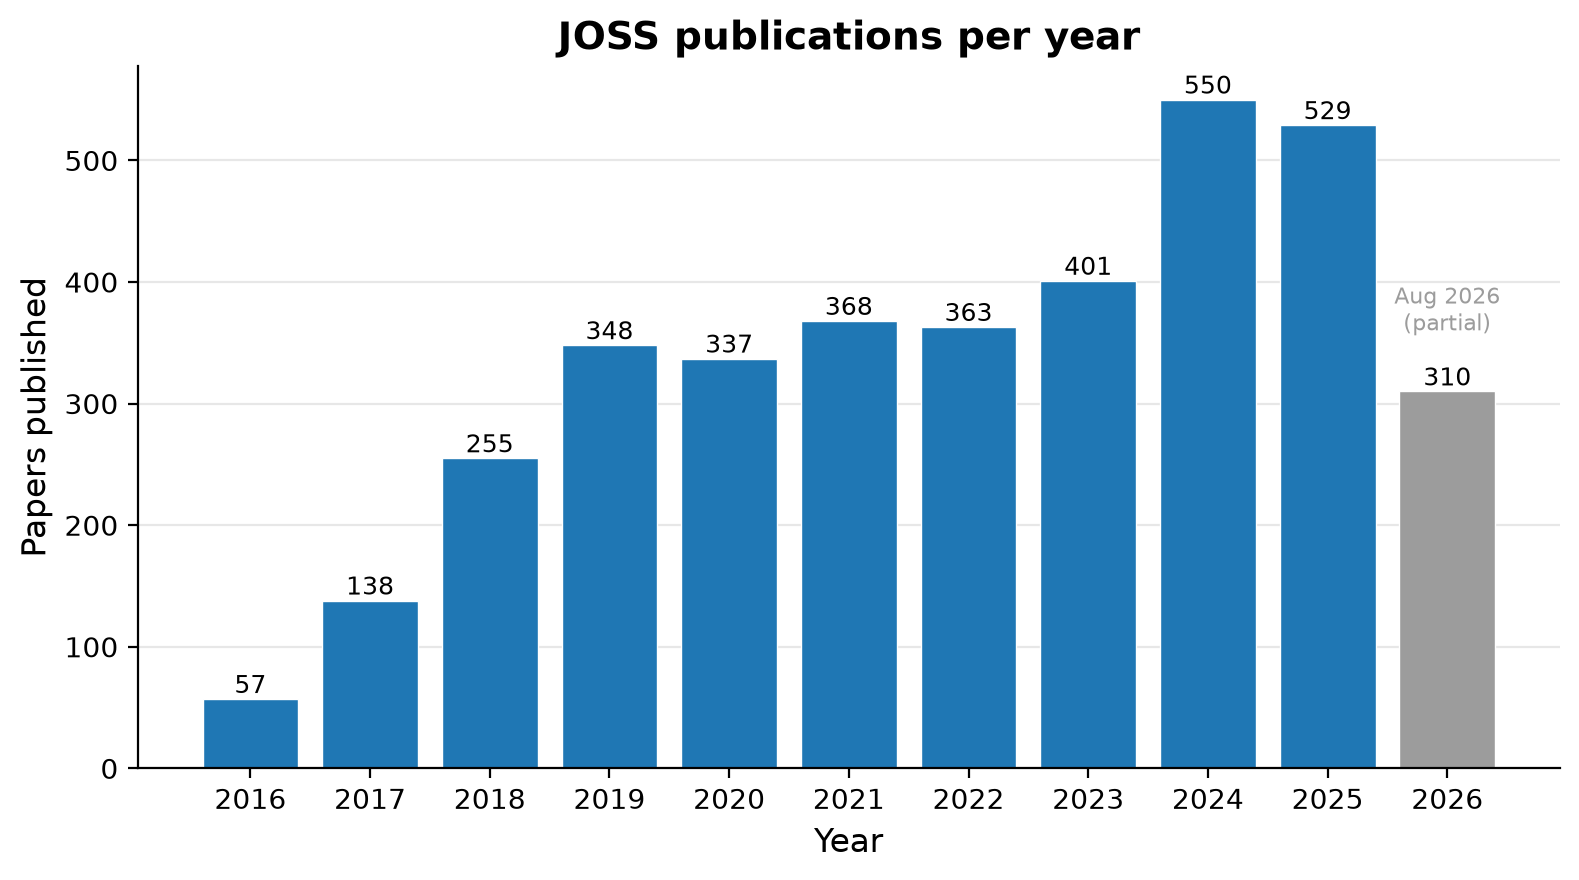
\includegraphics[width=0.43\textwidth]{joss-papers-per-year.png}
  \end{center}
  %
  \vspace{-1.32em}
  \begin{center}
    \emph{Most-cited articles}:\\[0.3em]
  \begin{tabular}{p{0.62\linewidth}@{\quad}cr}
    \textbf{Title} & \textbf{Date} & \textbf{Citations} \\
    \href{http://doi.org/10.21105/joss.01686}{Welcome to the Tidyverse} & 2019-11-21 & 20, 288 \\
    \href{http://doi.org/10.21105/joss.00861}{UMAP: Uniform Manifold Approximation and Projection} & 2018-09-02 & 9, 423 \\
    \href{http://doi.org/10.21105/joss.03021}{seaborn: statistical data visualization} & 2021-04-06 & 7, 034 \\
    \href{http://doi.org/10.21105/joss.03139}{performance: An R Package for Assessment, Comparison and Testing of Statistical Models} & 2021-04-21 & 5, 081 \\
  \end{tabular}
  \end{center}
  \vspace{0.15em}
  \begin{center}
    \emph{Most popular subject tracks} (publication share since 2023):\\[0.3em]
    \begin{tabular}{p{0.75\linewidth}@{\quad}r}
      \textbf{Biomedical, chemistry \& materials} & 23\% \\
      \textbf{Data science \& AI} & 21\% \\
      \textbf{Computer \& information science, mathematics} & 17\% \\
      \textbf{Earth sciences \& environment} & 13\% \\
    \end{tabular}
  \end{center}
  %
  Other tracks are: \textbf{Physics \& engineering}, \textbf{Astronomy \& space
  science}, \textbf{Social \& behavioural sciences}, and \textbf{Miscellaneous}. \\[0.5em]
  %
  After initial growth, submission and publication stabilised until 2024 where a new
  period of growth began, driven by generative AI facilitating rapid generation of code.
  \textbf{Increase in code is not increase in quality software}, however, placing a
  burden on journal editors and reviewers.
}

\column{0.5}
%
\block{Scope update: generative AI}{
  \textbf{In early 2026 JOSS
  \href{https://blog.joss.theoj.org/2026/01/preparing-joss-for-a-generative-ai-future}{updated
  its submission scope} in response to the rise of generative AI}: the original
  benchmarks were obsolete now code generation is cheap.
  JOSS now specifically evaluates \textbf{irreplaceable human contributions} rather
  than raw code output. Since these changes the pre-review rejection
  rate has climbed from \textasciitilde 27\% (2020--2024 average) to 48\% in
  2025 and 74\% so far in 2026:
  %
  \begin{center}
    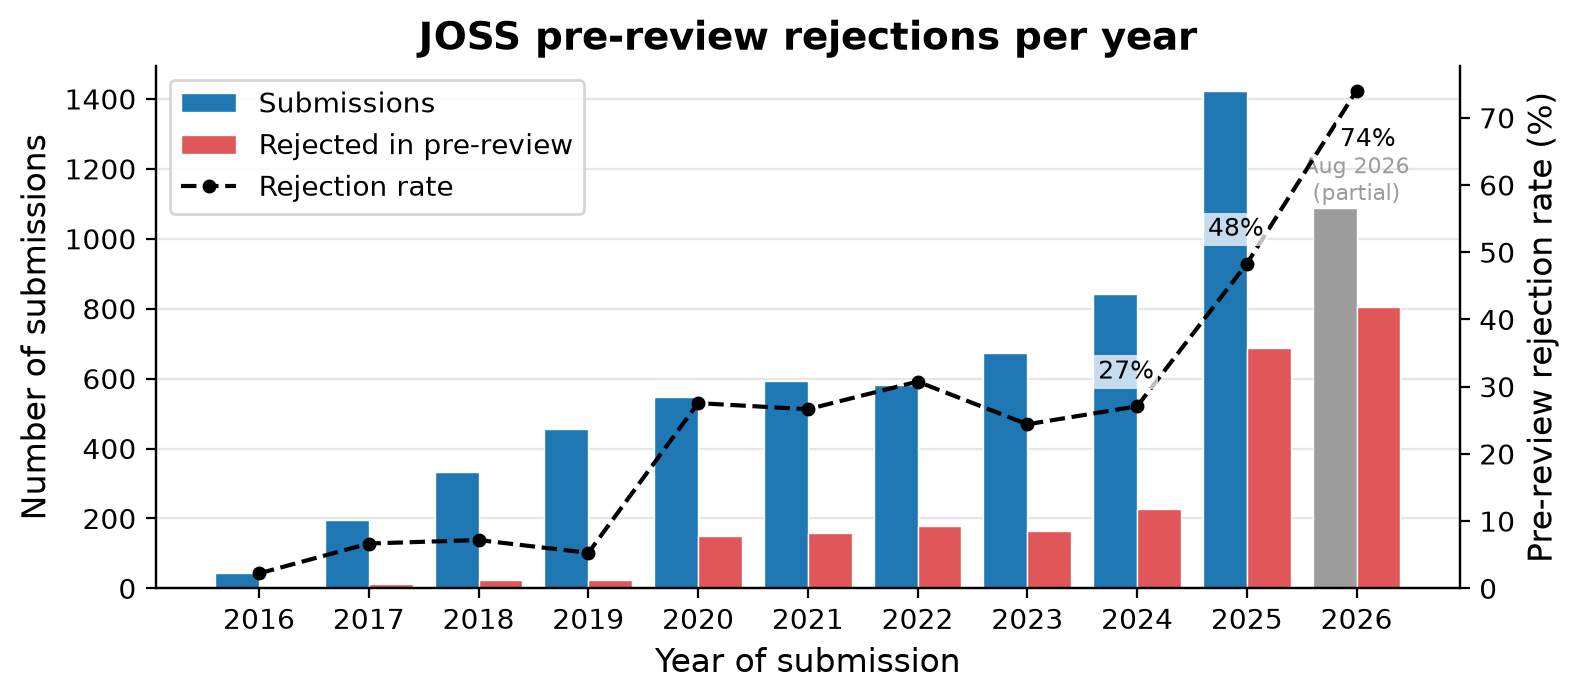
\includegraphics[width=0.45\textwidth]{joss-rejections-per-year.png}
  \end{center}
  \vspace{-1.0em}
  %
  Key changes in 2026:
  \begin{itemize}
    \item Development must \textbf{show iterative refinement} over time;
      ``code dumps'' and chunk replacements are desk-rejected.
    \item \textbf{Evidence of research impact} via
      publications, external adopters, and/or community engagement is required.
    \item Projects must show at least \textbf{six months of public
      development history} before submission.
    \item The paper must now include sections on: the current state of the field,
      software design, and research impact.
    \item An \textbf{AI-usage disclosure is mandatory} with authors (and reviewers)
      confirming human review of AI-assisted outputs.
  \end{itemize}
}

\block{Get involved}{
  \href{https://joss.readthedocs.io/en/latest/submitting.html}{\textbf{Publish your software!}}
  --- JOSS papers are deliberately brief: 750--1,750 words in a set format,
  so if your code is documented and tested a submission can be prepared quickly. \\
  \href{https://reviewers.joss.theoj.org/join}{\textbf{Volunteer to review!}}
  --- reviews are checklist-based with an iterative conversation on GitHub helping
  creators improve their software. \\
  \href{https://joss.theoj.org/about}{\textbf{Become an editor!}}
  --- find reviewers and guide submissions through review.  No open call,
  but if you have experience please reach out.
}

% \begin{subcolumns}
%   \subcolumn{0.45}
%   \block{JOSS homepage}{\begin{center}
%       \url{https://joss.theoj.org} \\
%       \includegraphics[width=0.15\textwidth]{joss-qr.png}
%   \end{center}}
%   \subcolumn{0.55}
  \block{About this poster}{
    Presented by \href{https://jackatkinson.net/}{Jack Atkinson}, Adam Tyson,
    Warrick Ball, and Daniel S.~Katz at the
    \emph{Tenth Annual Conference for Research Software Engineering}
    (RSECon26) at the University of Sheffield, UK, 9-11 Sep 2026.
    Scripts and data:
    \href{https://doi.org/10.5281/zenodo.2211124}{10.5281/zenodo.22111248} \\
    \begin{wrapfigure}[3]{r}{8.5cm}
      \vskip-1em\includegraphics[width=\linewidth]{by.png}
    \end{wrapfigure}
    Licensed CC-BY 4.0:
    \url{http://creativecommons.org/licenses/by/4.0/}
}
% \end{subcolumns}

% \block{Further information}
% {\begin{center}\begin{tabular}{p{20cm}|p{10cm}}
% %   & \textbf{JOSS homepage} \\
% %   & \url{https://joss.theoj.org} \\
%       Presented by Warrick Ball at the \emph{Ninth Annual Conference for Research Software Engineering}
%       (RSECon23) at the University of Warwick, 9-11 Sep 2025. \includegraphics[width=0.15\textwidth]{by.png} &
%       \textbf{JOSS homepage}
%        \\
% \end{tabular}\end{center}}
\end{columns}

% \begin{columns}

% % FIRST column
% \column{0.6}% Width set relative to text width

% \block{Large Column}{Text\\Text\\Text Text Text}
% \note{Note with default behavior}
% \note[targetoffsetx=12cm, targetoffsety=-1cm, angle=20, rotate=25]
% {Note \\ offset and rotated}

% % First column - second block
% \block{Block titles with enough text will automatically obey spacing requirements }
% {Text\\Text}

% % SECOND column
% \column{0.4}
% %Second column with first block’s top edge aligned with previous column’s top.

% % Second column - first block
% \block[titleleft]{Smaller Column}{Test}

% % Second column - second block
% \block[titlewidthscale=0.6, bodywidthscale=0.8]
% {Variable width title}{Block with smaller width.}

% % Second column - third block
% \block{}{Block with no title}

% % Second column - A collection of blocks in subcolumn environment
% \begin{subcolumns}
% \subcolumn{0.27} \block{1}{First block.} \block{2}{Second block}
% \subcolumn{0.4} \block{Sub-columns}{Sample subblocks\\Second subcolumn}
% \subcolumn{0.33} \block{4}{Fourth} \block{}{Final Subcolumn block}
% \end{subcolumns}
% \end{columns}
% \block[titleleft, titleoffsetx=2em, titleoffsety=1em, bodyoffsetx=2em,%
% bodyoffsety=-2cm, roundedcorners=10, linewidth=0mm, titlewidthscale=0.7,%
% bodywidthscale=0.9, bodyverticalshift=2cm, titleright]
% {Block outside of Columns}{Along with several options enabled}

\end{document}
